\documentclass[12pt]{beamer}

\usepackage{ucs}
\usepackage[utf8x]{inputenc}
\usepackage{beamerthemenirma}

\usepackage[australian]{babel}
\usepackage[T1]{fontenc}
\usepackage{graphicx}

\title{PODD Ontology Driven Database}
\author{Dr Peter Ansell}
\institute{University of Queensland}
\date{13 March 2012}

\begin{document}

\begin{frame}
\titlepage
\end{frame}

\begin{frame}{Outline}
  \tableofcontents
  % You might wish to add the option [pausesections]
\end{frame}

\section{Scientific experiments}

\begin{frame}
\frametitle{Scientific experiments}

\begin{itemize}
 \item Aim to test hypotheses in known, partially controlled situations
\pause
 \item Contain many variables
\pause
 \item Experiment variables are noted in workbooks
\end{itemize}

\end{frame}

\begin{frame}
\frametitle{Scientific workbooks}

\begin{itemize}
 \item Some common headings
\pause
 \item Structure can vary
\end{itemize}

\end{frame}

\section{Structured data}

\begin{frame}
\frametitle{Tables}

\begin{itemize}
 \item Two dimensional structure
\pause
 \item Suit simple relationships
\pause
 \item Single table not ideal for entire experiment
\end{itemize}

\end{frame}

\begin{frame}
\frametitle{Trees}

\begin{itemize}
 \item Everything has a common root
\pause
 \item Branches are independent of each other
\end{itemize}

\end{frame}

\section{PODD Ontology Driven Database}

\begin{frame}
\frametitle{PODD as a workbook}

\begin{itemize}
 \item Vital metadata about each experiment
\pause
 \item Variable number of headings and subheadings
\pause
 \item Acceptable use of headings and subheadings is configurable
\pause
 \item Each workbook is independent of other workbooks
\end{itemize}

\end{frame}


\begin{frame}
\frametitle{Ontologies to define structure}

\begin{itemize}
 \item Ontologies can be arbitrarily structured
\pause
 \item PODD has basic constraints
\begin{enumerate}
 \item Each ontology must have exactly one Project
 \item Each node must be connected to the Project through a series of ``part\_of'' links
 \item Each node can reference other nodes using ``refers\_to'' links
\end{enumerate}
\pause
\item Ontology defines acceptable structure without imposing a single schema on every workbook

\end{itemize}

\end{frame}

\begin{frame}
\frametitle{Phenomics ontology structure}

\begin{center}
 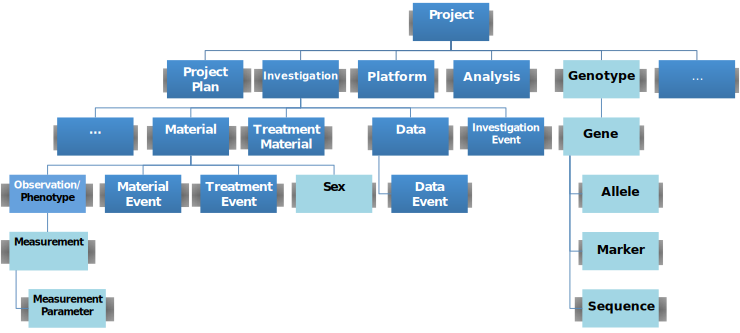
\includegraphics[scale=0.40,keepaspectratio=true]{./podd_ont.pdf}
 % podd_ont.pdf: 720x540 pixel, 72dpi, 25.40x19.05 cm, bb=0 0 720 540
\end{center}


\end{frame}


\end{document}

